
\section{targets.xml}

The targets file is used to define production and degradation constraints,
i.e. fluxes of metabolic \species{} or \macromolecule{}s that must be maintained
for the cell to be functional.

\subsection{Rationale}

In an RBA model, the production of machines (enzymes and process machines)
is automatically computed to sustain the metabolic fluxes and the production
of macromolecules necessary to achieve optimal growth rate.
However, in order to grow, the cell must produce more than just enzymes and ribosomes.
These production constraints are defined in targets.xml as fluxes or concentrations
that a cell must maintain in order to be functional.

Typical targets include molecules such as DNA, mRNAs, or housekeeping proteins
whose concentration must be maintained at all times.
Structural molecules contained in cell wall for example, must also be
maintained at a constant concentration.
A less obvious example are essential metabolites whose concentration
is high and well regulated, such as NADP/NADPH.\@
Defining a target concentration for NADP forces de novo production of NADP,
otherwise the model assumes that recycling existing NADP is sufficient to achieve any growth rate.
We suggest defining target concentrations for metabolites whenever metabolomic data are available.

In general, targets are defined as concentrations to maintain,
but it's also possible to specify absolute fluxes of production for metabolites or reactions.
A typical reaction flux that must be maintained is the production of maintenance ATP
(ATP used by secondary processes of the cell).

From the XML point of view, the definition of target constraints uses the same structure
as the density constraints.
In particular, the constraints may be equalities
(the concentration must be maintained to that exact value)
or inequalities (the concentration must be maintained between these bounds).

\subsection{RBATargets}
\label{sec:rba_targets}

The outermost part of the process file is an instance of class
\rbatargets, shown in Figure~\ref{fig:targets_doc}.

\begin{figure}
  \centering
  
\includegraphics[scale=0.8]{figures/targets_doc}
  \caption{XML structure of target document.}
\label{fig:targets_doc}
\end{figure}

\rbatargets{} has no simple attributes.
It contains 3 \textbf{ListOfTargetSpecies}.
These targets allow to define metabolic \species{} or \macromolecule{} fluxes.
One is for production fluxes, another for degradation fluxes.
The last list is for maintaining a target at a given concentration.
The difference with a simple production flux is that keeping a target at a
concentration depends on growth rate.
More precisely, the flux needed to keep the concentration is
the growth rate multiplied by the target concentration.
Note that all fluxes must be positive.
If the target is a \macromolecule, production/degradation can only occur
if the \processings{} section of some \process{} defines how the
\macromolecule{} is actually produced/degraded.

It contains a \textbf{ListOfTargetReactions}.
It is also possible to define target fluxes as reaction fluxes.
These targets add constraints on the flux of a specific metabolic \reaction.
In this case, fluxes may be positive or negative.


\subsection{TargetSpecies}
\label{sec:target_species}

The \targetspecies{} class defines constraints for a species flux
(Fig.~\ref{fig:targets_doc}).
It inherits \targetvalue{} for the constraint definition part, allowing for
equality or inequality constraints.

\paragraph{The \textit{species} attribute}
The \textbf{species} attribute is a string that must match the identifier
of a metabolic \species{} or a \macromolecule{}.
Note that the \macromolecule{} must be broken down into metabolite costs
through the \processings{} section of some \process{}.
Otherwise no cost will be applied.


\subsection{TargetReaction}
\label{sec:target_reaction}

The \targetreaction{} class defines constraints for a reaction flux
(Fig.~\ref{fig:targets_doc}).
It inherits \targetvalue{} for the constraint definition part, allowing for
equality or inequality constraints.

\paragraph{The \textit{reaction} attribute}
The \textbf{reaction} attribute is a string that must match the identifier
of a metabolic \reaction{}.

\subsection{Examples}

Most targets in an RBA model are concentration targets for DNA production,
mRNA production, housekeeping protein production, de novo metabolite
production, by specifying a concentration that must be maintained
(Fig.~\ref{fig:targets_ex_1} and \ref{fig:targets_ex_2}).

The second class of targets are fluxes related to degradation.
For example, our \textit{B. subtilis} model explicitly accounts for mRNA
degradation.
As a result, there are 3 target fluxes associated with mRNAs:
a flux associated with the target concentration to maintain,
a flux indicating how many molecules are degraded by seconds
(how mRNAs are degraded is defined in processes.xml),
and an absolute production flux that exactly compensates degradation
(Fig.~\ref{fig:targets_ex_1}).

The third class of targets are targets that reference reactions instead of
metabolic species or macromolecules.
Maintenance ATP is one of the most common examples,
but there are a lot of contextual requirements that can be written in this form,
such as flagella movement,
response to stresses such as oxidative stresses causing NADPH consumption.

\begin{figure}
  \centering
  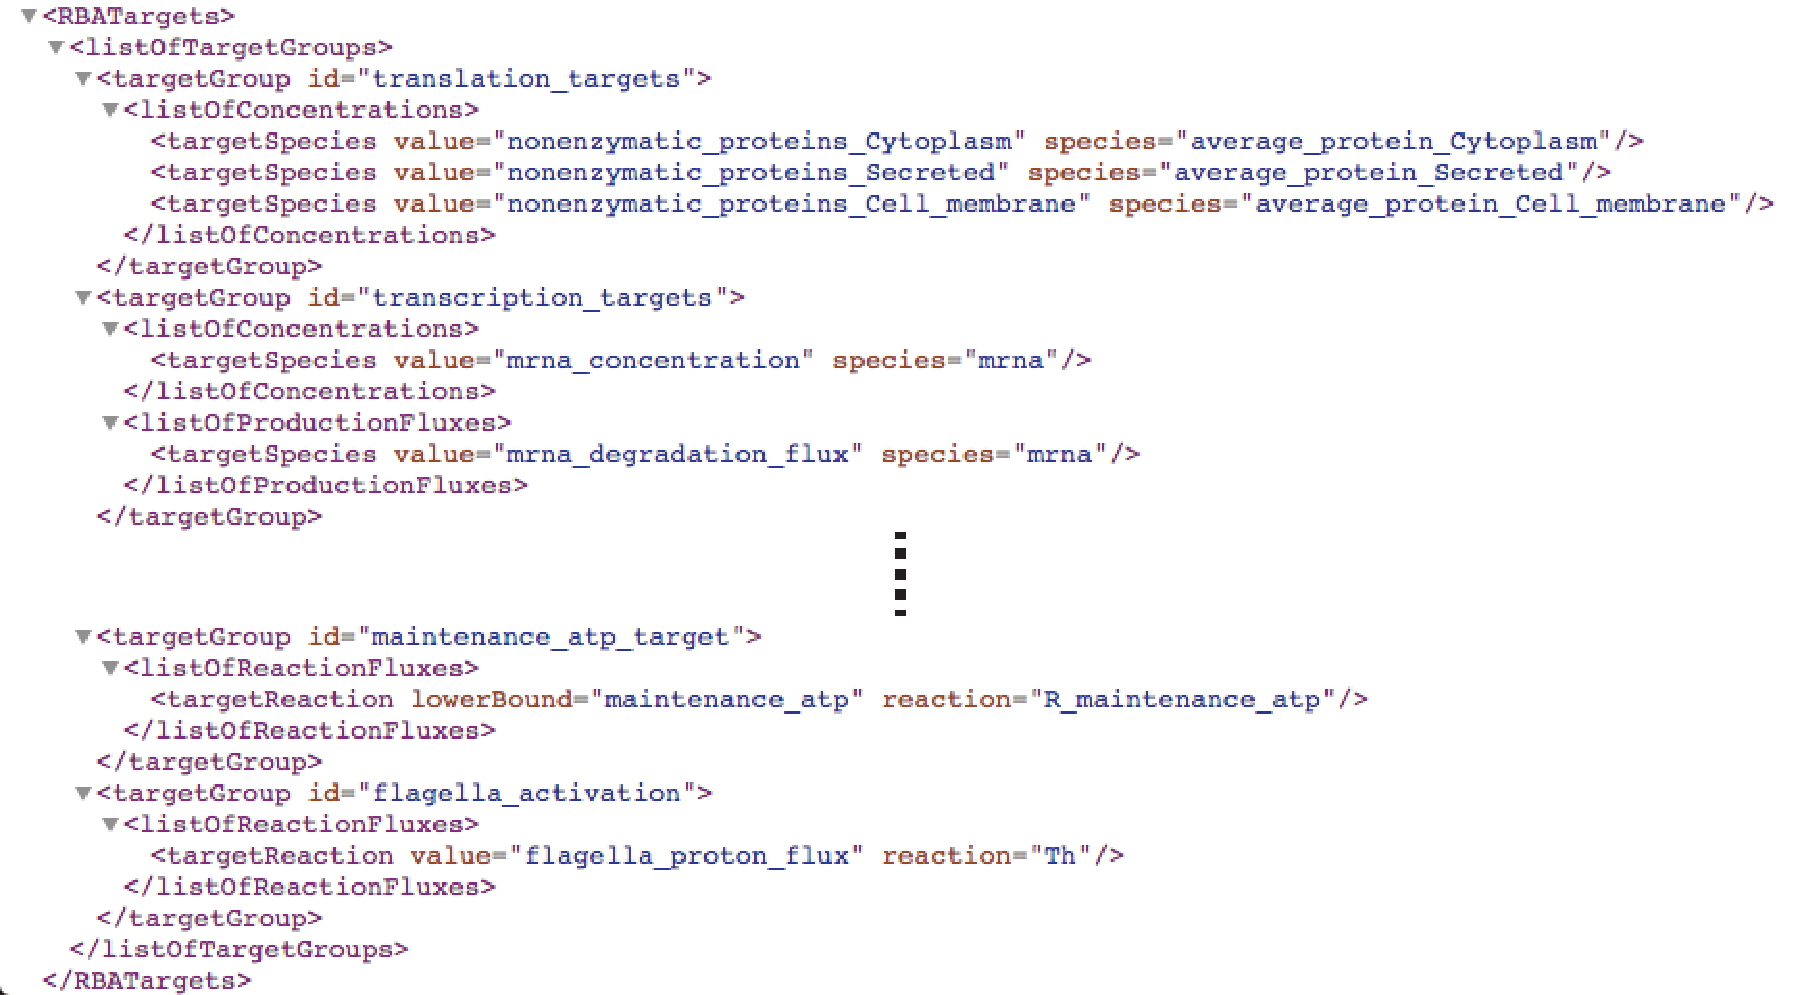
\includegraphics[scale=0.6]{figures/targets_ex_1}
  \caption{targets.xml from a hand-curated model for the
  model bacteria \textit{B. subtilis}.
  Large parts of the files where removed for brevity.
  The first 3 targetSpecies encompass all nonenzymatic proteins that must be
  produced by the cell for housekeeping purposes.
  mRNAs have two production constraints:
  the first contraint defines a flux that must be generated in order to
  maintain their concentration,
  the second constraint defines a flux that must be generated in order to
  compensate degradation (defined later in the file).
  Finally, there are two example of reaction targets:
  a lowerBound for maintainance ATP production,
  and a set bound for the reaction controlling flagella movement.}
  \label{fig:targets_ex_1}
\end{figure}

\begin{figure}
  \centering
  \includegraphics[scale=0.6]{figures/targets_ex_2}
  \caption{targets.xml from the minimal model.
  We pool all non-machine production requirements in a
  generic biomass production requirement.}
  \label{fig:targets_ex_2}
\end{figure}
